\begin{enumerate}[label=\thesubsection.\arabic*, ref=\thesubsection.\theenumi]
	\item 		Find the values of $x$ and $y$ so that the vectors
$2\hat{i}+3\hat{j}$
and 
$x\hat{i}+y\hat{j}$
are equal.
\\
\solution
%\renewcommand{\theequation}{\theenumi}
\begin{enumerate}[label=\thesubsection.\arabic*.,ref=\thesubsection.\theenumi]
%\numberwithin{equation}{enumi}
\item The direction vector of $AB$ is defined as
		\begin{align}
			\vec{B}-
			\vec{A}
		\end{align}
Find the direction vectors of $AB, BC$ and $CA$.
\\
\solution 
\begin{enumerate} 
\item  The Direction vector of $AB$ is 
	\begin{align}  \vec{B} - \vec{A} 
		=\myvec{ -4\\ 6 } - \myvec{ 1\\ -1 }
 = \myvec{ -4 - 1\\ 6 - (-1) } = \myvec{ -5\\ 7 }
		\label{eq:app-geo-dir-vec-ab}
 \end{align}
\item The Direction vector of $BC$ is
	\begin{align} \vec{C} - \vec{B}=\myvec{ -3\\ -5} - \myvec{ -4\\ 6 }
 = \myvec{ -3 - (-4)\\ -5 - 6 } = \myvec{1\\ -11 }
		\label{eq:app-geo-dir-vec-bc}
  \end{align}
  \item  The Direction vector of $CA$  is
	  \begin{align}  \vec{A} - \vec{C} =\myvec{ 1\\ -1 }-\myvec{ -3\\ -5}
 = \myvec{ 1 - (-3)\\ -1 - (-5) } = \myvec{ 4\\ 4 }
		\label{eq:app-geo-dir-vec-ca}
  \end{align}
 \end{enumerate}
%	\solution 
\begin{enumerate} 
\item  The Direction vector of $AB$ is 
	\begin{align}  \vec{B} - \vec{A} 
		=\myvec{ -4\\ 6 } - \myvec{ 1\\ -1 }
 = \myvec{ -4 - 1\\ 6 - (-1) } = \myvec{ -5\\ 7 }
		\label{eq:geo-dir-vec-ab}
 \end{align}
\item The Direction vector of $BC$ is
	\begin{align} \vec{C} - \vec{B}=\myvec{ -3\\ -5} - \myvec{ -4\\ 6 }
 = \myvec{ -3 - (-4)\\ -5 - 6 } = \myvec{1\\ -11 }
		\label{eq:geo-dir-vec-bc}
  \end{align}
  \item  The Direction vector of $CA$  is
	  \begin{align}  \vec{A} - \vec{C} =\myvec{ 1\\ -1 }-\myvec{ -3\\ -5}
 = \myvec{ 1 - (-3)\\ -1 - (-5) } = \myvec{ 4\\ 4 }
		\label{eq:geo-dir-vec-ca}
  \end{align}
 \end{enumerate}


	\item The length of side $BC$ is 
		\label{prob:side-length}
		\begin{align}
			c = \norm{\vec{B}-\vec{A}} \triangleq \sqrt{\brak{\vec{B}-\vec{A}}^{\top}\brak{\vec{B}-\vec{A}}}
		\end{align}
		where
		\begin{align}
			\vec{A}^{\top}\triangleq\myvec{1 & -1}
		\end{align}
		Similarly, 
		\begin{align}
b = \norm{\vec{C}-\vec{B}},\,
a = \norm{\vec{A}-\vec{C}}
		\end{align}
		Find $a, b, c$.
\begin{enumerate}
	\item 
	From 	
		\eqref{eq:app-geo-dir-vec-ab},
\begin{align}
\vec{A}-\vec{B} &= \myvec{5\\-7}, \\
\implies 	c &= 	\norm{\vec{B}-\vec{A}} = \norm{\vec{A}-\vec{B}} 
	\\
	&= \sqrt{\myvec{5 & -7}\myvec{5\\-7}}
= \sqrt{\brak{5}^2 +\brak{7}^2}\\
	&=\sqrt{74}
		\label{eq:app-geo-norm-ab}
\end{align}
	\item Similarly, from 
		\eqref{eq:app-geo-dir-vec-bc},
\begin{align}
	a &= \norm{\vec{B}-\vec{C}} 
	= \sqrt{\myvec{-1 & 11}\myvec{-1\\11}}
\\
&= \sqrt{\brak{1}^2+\brak{11}^2}
	= \sqrt{122}
		\label{eq:app-geo-norm-bc}
\end{align}
and
		from 		\eqref{eq:app-geo-dir-vec-ca},
	\item 
		\begin{align}
			b &= \norm{\vec{A}-\vec{C}} = \sqrt{\myvec{4 & 4}\myvec{4\\4}}
\\
&= \sqrt{\brak{4}^2+\brak{4}^2}
	=\sqrt{32}
		\label{eq:app-geo-norm-ca}
\end{align}
\end{enumerate}
%  \\            
  %\\ \solution 
\begin{align}
    \vec{A}-\vec{F}&=\myvec{1\\-1}-\myvec{\frac{-3}{2}\\\frac{5}{2}}
    =\myvec{\frac{5}{2}\\\frac{-7}{2}}
    \\
    \vec{E}-\vec{D}&=\myvec{-1\\-3}-\myvec{\frac{-7}{2}\\\frac{1}{2}}
    =\myvec{\frac{5}{2}\\\frac{-7}{2}}
    \\
	\implies	\vec{A}-\vec{F} &= \vec{E}-\vec{D}
\end{align}
See \figref{fig:Triangle-pgm}, 
\begin{figure}
\centering
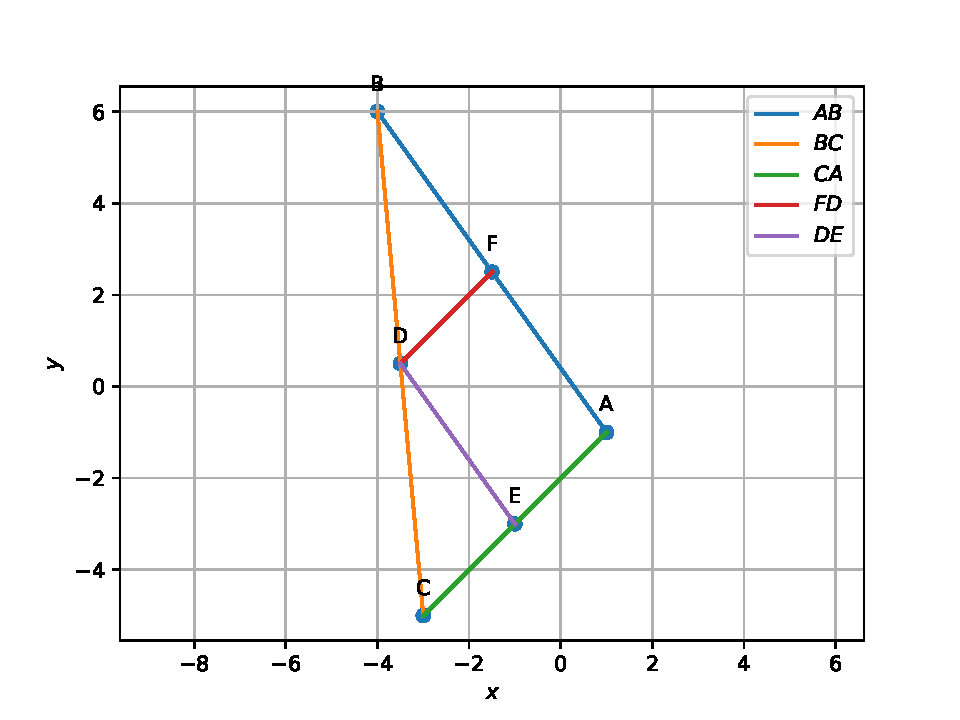
\includegraphics[width=0.75\columnwidth]{figs/triangle/pgm.pdf}
\caption{$AFDE$ forms a parallelogram in triangle ABC}
\label{fig:Triangle-pgm}
\end{figure}






















\item   Points $\vec{A}, \vec{B}, \vec{C}$ are defined to be collinear if 
		\begin{align}
			\label{eq:app-app-line-rank}
			\rank{\myvec{1 & 1 & 1 \\ \vec{A}& \vec{B}&\vec{C}}} = 2
		\end{align}
Are the given points in
			\eqref{eq:app-tri-pts}
collinear?
\\
\solution 
From 
			\eqref{eq:app-tri-pts},
\begin{align}
    \label{eq:app-1.1.3,2}
\myvec{
    1 & 1 & 1\\
    \vec{A} & \vec{B} & \vec{C} \\
    } 
    =
    %\label{eq:app-matthrowoperations}
    \myvec{
    1 & 1 & 1
    \\
    1 & -4 & -3
    \\
    -1 & 6 & -5
    }
     \xleftrightarrow[]{R_3 \leftarrow R_3+R_2}
    \myvec{
    1 & 1 & 1
    \\
    1 & -4 & -3
    \\
    0 & 2 & -8 
    }
    \\
     \xleftrightarrow[]{R_2\leftarrow R_1-R_2}
    \myvec{
    1 & 1 & 1
    \\
    0 & 5 & 4
    \\
    0 & 2 & -8 
    }
     \xleftrightarrow[]{R_3\leftarrow R_3-\frac{2}{5}R_2}
    \myvec{
    1 & 1 & 1
    \\
    0 & 5 & 4
    \\
    0 & 0 & \frac{-48}{5}
    }
\end{align}
There are no zero rows. So,
\begin{align}
    \text{rank}\myvec{
    1 & 1 & 1\\
    \vec{A} & \vec{B} & \vec{C} \\
    } &= 3 
\end{align}  
Hence,  the points $\vec{A},\vec{B},\vec{C}$ are not collinear. 
This is visible in 
\figref{fig1:Triangle}.
\begin{figure}[H]
\centering
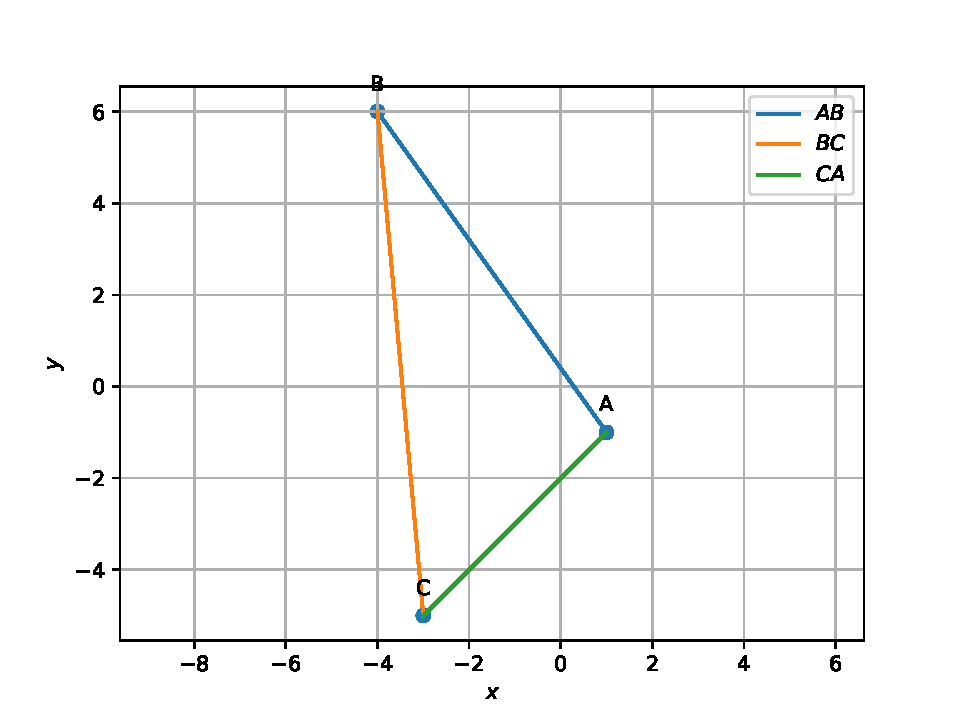
\includegraphics[width=0.75\columnwidth]{figs/triangle/vector.pdf}
\caption{$\triangle ABC$}
\label{fig1:Triangle}
\end{figure}
% \\		\\ \solution 
\begin{align}
    \vec{A}-\vec{F}&=\myvec{1\\-1}-\myvec{\frac{-3}{2}\\\frac{5}{2}}
    =\myvec{\frac{5}{2}\\\frac{-7}{2}}
    \\
    \vec{E}-\vec{D}&=\myvec{-1\\-3}-\myvec{\frac{-7}{2}\\\frac{1}{2}}
    =\myvec{\frac{5}{2}\\\frac{-7}{2}}
    \\
	\implies	\vec{A}-\vec{F} &= \vec{E}-\vec{D}
\end{align}
See \figref{fig:Triangle-pgm}, 
\begin{figure}
\centering
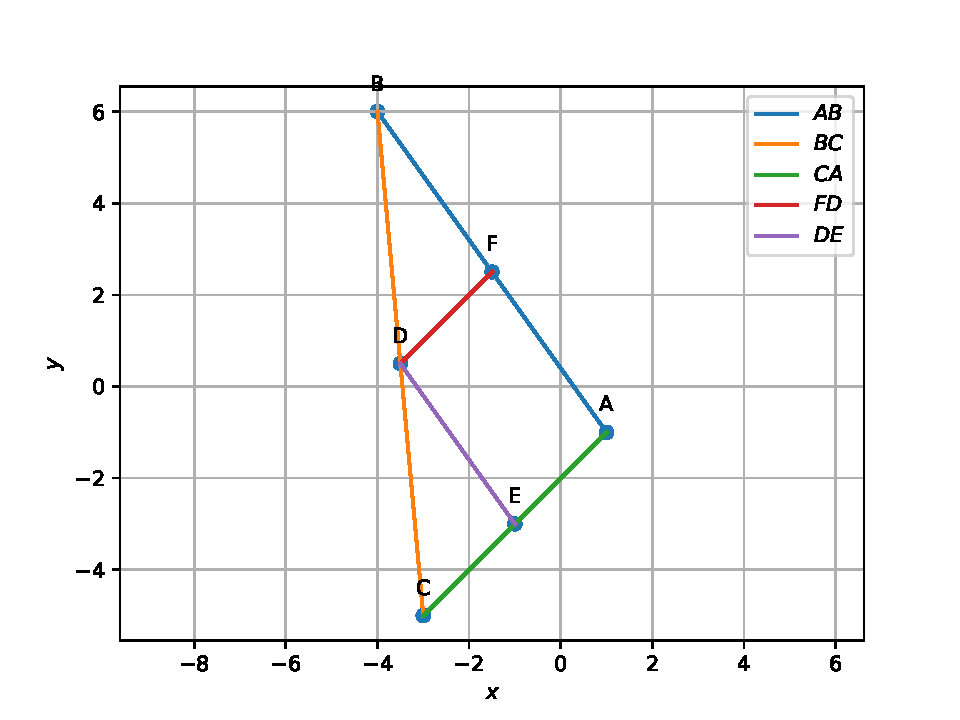
\includegraphics[width=0.75\columnwidth]{figs/triangle/pgm.pdf}
\caption{$AFDE$ forms a parallelogram in triangle ABC}
\label{fig:Triangle-pgm}
\end{figure}






















\item The parameteric form of the equation  of $AB$ is 
		\begin{align}
			\label{eq:app-geo-param}
			\vec{x}=\vec{A}+k\vec{m} \quad k \ne 0,
		\end{align}
		where
		\begin{align}
\vec{m}=\vec{B}-\vec{A}
		\end{align}
is the direction vector of $AB$.
Find the parameteric equations of $AB, BC$ and $CA$.
\\
\solution
From 
			\eqref{eq:app-geo-param} and
		\eqref{eq:app-geo-dir-vec-ab},
the parametric equation for $AB$ is given by
\begin{align}
AB: \vec{x} = &\myvec{1\\-1} + k \myvec{-5\\7}
\end{align}
Similarly, from 
		\eqref{eq:app-geo-dir-vec-bc} and
		\eqref{eq:app-geo-dir-vec-ca},
\begin{align}
BC: \vec{x} = &\myvec{-4\\6} + k \myvec{1\\-11}\\
CA: \vec{x} = &\myvec{-3\\-5} + k \myvec{4\\4}
\end{align}

%		\\ \solution 
\begin{align}
    \vec{A}-\vec{F}&=\myvec{1\\-1}-\myvec{\frac{-3}{2}\\\frac{5}{2}}
    =\myvec{\frac{5}{2}\\\frac{-7}{2}}
    \\
    \vec{E}-\vec{D}&=\myvec{-1\\-3}-\myvec{\frac{-7}{2}\\\frac{1}{2}}
    =\myvec{\frac{5}{2}\\\frac{-7}{2}}
    \\
	\implies	\vec{A}-\vec{F} &= \vec{E}-\vec{D}
\end{align}
See \figref{fig:Triangle-pgm}, 
\begin{figure}
\centering
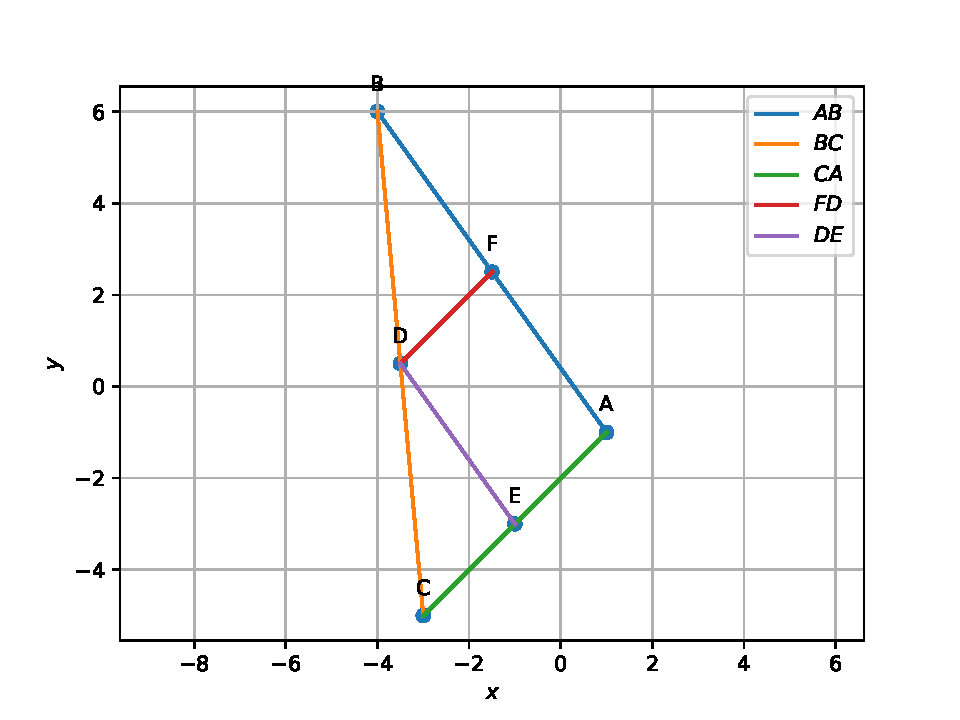
\includegraphics[width=0.75\columnwidth]{figs/triangle/pgm.pdf}
\caption{$AFDE$ forms a parallelogram in triangle ABC}
\label{fig:Triangle-pgm}
\end{figure}






















\item The normal form of the equation of $AB$  is 
		\begin{align}
			\label{eq:app-geo-normal}
			\vec{n}^{\top}\brak{	\vec{x}-\vec{A}} = 0
		\end{align}
		where 
		\begin{align}
			\vec{n}^{\top}\vec{m}&=\vec{n}^{\top}\brak{\vec{B}-\vec{A}} = 0
			\\
			\text{or, } \vec{n}&=\myvec{0 & 1 \\ -1 & 0} \vec{m}
			\label{eq:app-geo-norm-vec}
		\end{align}
Find the normal form of the equations of $AB, BC$ and $CA$.
\\
\solution
\begin{enumerate}
	\item
From
		\eqref{eq:app-geo-dir-vec-bc}, 
the direction vector of side $\vec{BC}$ is
\begin{align}
\vec{m}
	&=\myvec{1\\-11}
	\\
\implies \vec{n} &= \myvec{0 & 1\\
  -1 & 0}\myvec{1\\-11}
 = \myvec{-11\\-1}
		\label{eq:app-geo-norm-vec-bc}
\end{align}
from 
			\eqref{eq:app-geo-norm-vec}.
Hence, from 
			\eqref{eq:app-geo-normal},
the normal equation of side $BC$ is 
\begin{align}
	\vec{n}^{\top}\brak{	\vec{x}-\vec{B}} &= 0
			\\
\implies    \myvec{-11 & -1}\vec{x}&=\myvec{-11 & -1}\myvec{-4\\6}\\
    \implies
BC: \quad    \myvec{11 & 1}\vec{x}&=-38
\end{align}
\item Similarly, for $AB$,
from 
		\eqref{eq:app-geo-dir-vec-ab}, 
\begin{align}
	\vec{m} &= \myvec{-5\\7}
	\\
\implies        \vec{n} 
                &= \myvec{0&1\\-1&0}\myvec{-5\\7}
                = \myvec{7\\5}
		\label{eq:app-geo-norm-vec-ab}
\end{align}
and 
\begin{align}
	\vec{n}^{\top}\brak{	\vec{x}-\vec{A}} &= 0
	\\
	\implies
                AB: \quad  \vec{n}^{\top}\vec{x} &= \myvec{7&5}\myvec{1\\-1}\\    
       \implies\myvec{7&5}\vec{x} &= 2
\end{align}
\item For 
$CA$, 
from 
		\eqref{eq:app-geo-dir-vec-ca}, 
\begin{align}
\vec{m} &= \myvec{1 \\ 1}
\\
		\label{eq:app-geo-norm-vec-ca}
\implies \vec{n} 
&= \myvec{0&1 \\ -1&0}\myvec{1 \\ 1}
= \myvec{1 \\ -1}\\
\\
\implies	\vec{n}^{\top}\brak{	\vec{x}-\vec{C}} &= 0
\\
\implies \myvec{1&-1}{\vec{x}} &= \myvec{1&-1}\myvec{-3 \\ -5} 
= 2 
\end{align}
\end{enumerate}

%\begin{enumerate}
	\item
From
		\eqref{eq:geo-dir-vec-bc}, 
the direction vector of side $\vec{BC}$ is
\begin{align}
\vec{m}
	&=\myvec{1\\-11}
	\\
\implies \vec{n} &= \myvec{0 & 1\\
  -1 & 0}\myvec{1\\-11}
 = \myvec{-11\\-1}
		\label{eq:geo-norm-vec-bc}
\end{align}
from 
			\eqref{eq:geo-norm-vec}.
Hence, from 
			\eqref{eq:geo-normal},
the normal equation of side $BC$ is 
\begin{align}
	\vec{n}^{\top}\brak{	\vec{x}-\vec{B}} &= 0
			\\
\implies    \myvec{-11 & -1}\vec{x}&=\myvec{-11 & -1}\myvec{-4\\6}\\
    \implies
BC: \quad    \myvec{11 & 1}\vec{x}&=-38
\end{align}
\item Similarly, for $AB$,
from 
		\eqref{eq:geo-dir-vec-ab}, 
\begin{align}
	\vec{m} &= \myvec{-5\\7}
	\\
\implies        \vec{n} 
                &= \myvec{0&1\\-1&0}\myvec{-5\\7}
                = \myvec{7\\5}
		\label{eq:geo-norm-vec-ab}
\end{align}
and 
\begin{align}
	\vec{n}^{\top}\brak{	\vec{x}-\vec{A}} &= 0
	\\
	\implies
                AB: \quad  \vec{n}^{\top}\vec{x} &= \myvec{7&5}\myvec{1\\-1}\\    
       \implies\myvec{7&5}\vec{x} &= 2
\end{align}
\item For 
$CA$, 
from 
		\eqref{eq:geo-dir-vec-ca}, 
\begin{align}
\vec{m} &= \myvec{1 \\ 1}
\\
		\label{eq:geo-norm-vec-ca}
\implies \vec{n} 
&= \myvec{0&1 \\ -1&0}\myvec{1 \\ 1}
= \myvec{1 \\ -1}\\
\\
\implies	\vec{n}^{\top}\brak{	\vec{x}-\vec{C}} &= 0
\\
\implies \myvec{1&-1}{\vec{x}} &= \myvec{1&-1}\myvec{-3 \\ -5} 
= 2 
\end{align}
\end{enumerate}


\item The area of $\triangle ABC$ is defined as
		\begin{align}
			\label{eq:app-tri-area-cross}
			\frac{1}{2}\norm{{\brak{\vec{A}-\vec{B}}\times \brak{\vec{A}-\vec{C}}}}
		\end{align}
		where
		\begin{align}
			\vec{A}\times\vec{B} \triangleq \mydet{1 & -4 \\-1 & 6}
		\end{align}
		Find the area of $\triangle ABC$.\\
\solution
From
		\eqref{eq:app-geo-dir-vec-ab}
		and
		\eqref{eq:app-geo-dir-vec-ca},
\begin{align}
	\vec{A}-\vec{B}=\myvec{5\\-7},
	\vec{A}-\vec{C}&=\myvec{4\\4}\\
\implies (\vec{A}-\vec{B})\times(\vec{A}-\vec{C}) &=\mydet{5 & 4\\-7 & 4}\\
&=5\times 4-4\times (-7)\\&=48\\
\implies\frac{1}{2}\norm{(\vec{A}-\vec{B})\times(\vec{A}-\vec{C})}&=\frac{48}{2}=24
\end{align}
which is the desired area.

%  		\\ \solution 
\begin{align}
    \vec{A}-\vec{F}&=\myvec{1\\-1}-\myvec{\frac{-3}{2}\\\frac{5}{2}}
    =\myvec{\frac{5}{2}\\\frac{-7}{2}}
    \\
    \vec{E}-\vec{D}&=\myvec{-1\\-3}-\myvec{\frac{-7}{2}\\\frac{1}{2}}
    =\myvec{\frac{5}{2}\\\frac{-7}{2}}
    \\
	\implies	\vec{A}-\vec{F} &= \vec{E}-\vec{D}
\end{align}
See \figref{fig:Triangle-pgm}, 
\begin{figure}
\centering
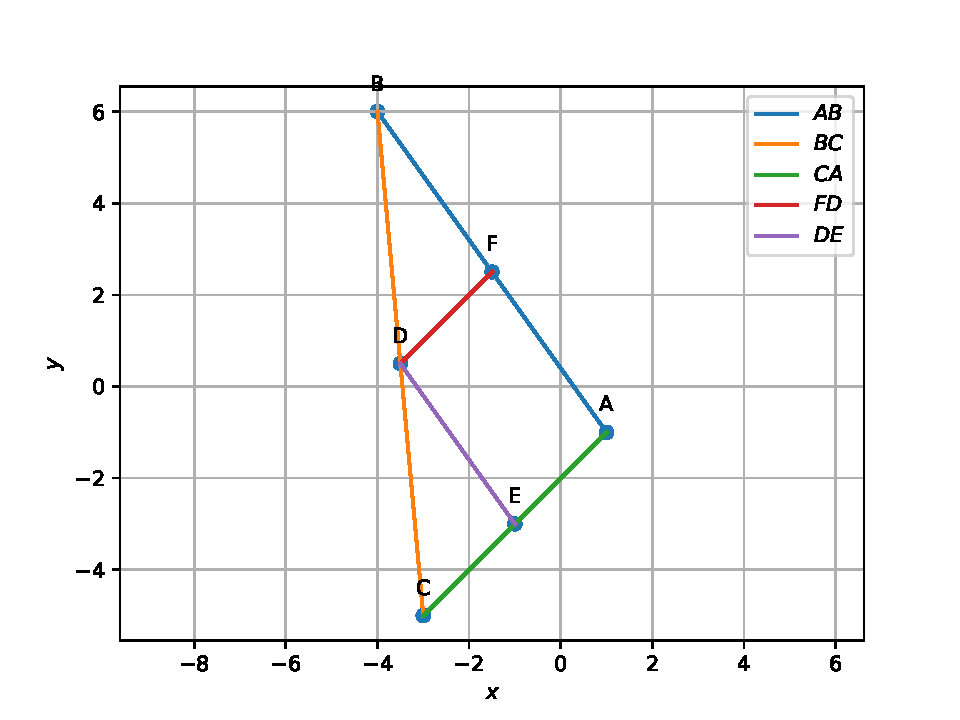
\includegraphics[width=0.75\columnwidth]{figs/triangle/pgm.pdf}
\caption{$AFDE$ forms a parallelogram in triangle ABC}
\label{fig:Triangle-pgm}
\end{figure}






















	\item Find the angles $A, B, C$ if 
%    \label{prop:angle2d}
  \begin{align}
    \label{eq:app-angle2d}
			\cos A \triangleq 
\frac{\brak{\vec{B}-\vec{A}}^{\top}{\vec{C}-\vec{A}}}{\norm{\vec{B}-\vec{A}}\norm{\vec{C}-\vec{A}}}
  \end{align}\\
  \solution
\begin{enumerate}
	\item From 
		\eqref{eq:app-geo-dir-vec-ab},
		\eqref{eq:app-geo-dir-vec-ca},
		\eqref{eq:app-geo-norm-ab}
		and
		\eqref{eq:app-geo-norm-ca}
\begin{align}
	(\vec{B}-\vec{A})^{\top}(\vec{C}-\vec{A})&=\myvec{-5&7}\myvec{-4\\-4}\\
	&=-8
	\\
	\implies
	\cos{A}&= \frac{-8}{\sqrt{74} \sqrt{32}}
	= \frac{-1}{\sqrt{37}}\\
	\implies A&=\cos^{-1}{\frac{-1}{\sqrt{37}}}
\end{align}
	\item From 
		\eqref{eq:app-geo-dir-vec-ab},
		\eqref{eq:app-geo-dir-vec-bc},
		\eqref{eq:app-geo-norm-ab}
		and
		\eqref{eq:app-geo-norm-bc}
\begin{align}
	(\vec{C}-\vec{B})^{\top}(\vec{A}-\vec{B})&=\myvec{1&-11}\myvec{5\\-7}\\
	&= 82
	\\
	\implies
	\cos{B}&= \frac{82}{\sqrt{74} \sqrt{122}}
	= \frac{41}{\sqrt{2257}}\\
	\implies B&=\cos^{-1}{\frac{41}{\sqrt{2257}}}
\end{align}
	\item From 
		\eqref{eq:app-geo-dir-vec-bc},
		\eqref{eq:app-geo-dir-vec-ca},
		\eqref{eq:app-geo-norm-bc}
		and
		\eqref{eq:app-geo-norm-ca}
\begin{align}
	(\vec{A}-\vec{C})^{\top}(\vec{B}-\vec{C})&=\myvec{4&4}\myvec{-1\\11}\\
	&=40
	\\
\implies	\cos{C}&= \frac{40}{\sqrt{32} \sqrt{122}}
	= \frac{5}{\sqrt{61}}\\
	\implies C&=\cos^{-1}{\frac{5}{\sqrt{61}}}
\end{align}

\end{enumerate}
%  	\\ \solution 
\begin{align}
    \vec{A}-\vec{F}&=\myvec{1\\-1}-\myvec{\frac{-3}{2}\\\frac{5}{2}}
    =\myvec{\frac{5}{2}\\\frac{-7}{2}}
    \\
    \vec{E}-\vec{D}&=\myvec{-1\\-3}-\myvec{\frac{-7}{2}\\\frac{1}{2}}
    =\myvec{\frac{5}{2}\\\frac{-7}{2}}
    \\
	\implies	\vec{A}-\vec{F} &= \vec{E}-\vec{D}
\end{align}
See \figref{fig:Triangle-pgm}, 
\begin{figure}
\centering
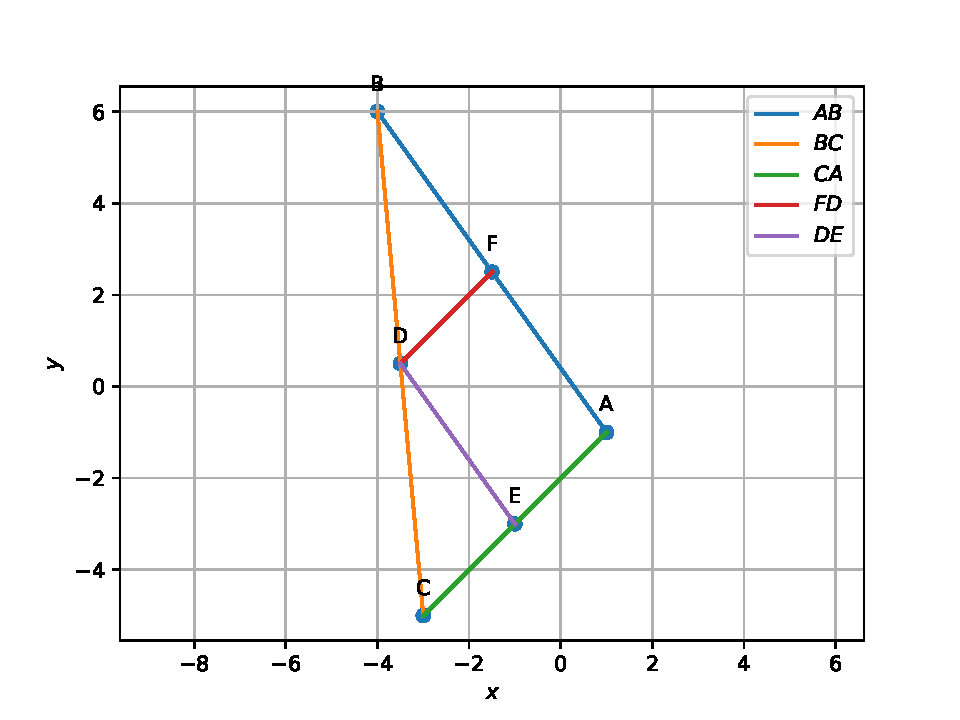
\includegraphics[width=0.75\columnwidth]{figs/triangle/pgm.pdf}
\caption{$AFDE$ forms a parallelogram in triangle ABC}
\label{fig:Triangle-pgm}
\end{figure}






















All codes for this section are available at
\begin{lstlisting}
	codes/triangle/sides.py
\end{lstlisting}
\end{enumerate}

\item Find the values of $x, y, z$ so that the vectors 
$x\hat{i}+2\hat{j}+z\hat{k}$
and 
$2\hat{i}+y\hat{j}+\hat{k}$
are equal.
\item Find the sum of the vectors $\vec{a}=\hat{i}-2\hat{j}+\hat{k}$,  $\vec{b}=-2\hat{i}+4\hat{j}+5\hat{k}$ and $\vec{c}=\hat{i}-6\hat{j}-7\hat{k}$.
\item Find the slope of a line,  which passes through the origin and the mid point of the line segment joining the points $\vec{P}$(0, -4) and $\vec{B}$(8, 0).
\label{chapters/11/10/1/5}
	\\
	\solution
The direction vector
\begin{align}
	\vec{B}-\vec{A}
	=
	\myvec{
  h-x_1\\
  k-y_1
  }
   \equiv
	\myvec{
1\\
	\frac{ k-y_1}{h-x_1}
  }
  \\
	\implies m = 
	\frac{ k-y_1}{h-x_1},
\end{align}
yielding the desired result.

\item Find the angle between x-axis and the line joining points (3, -1) and (4, -2).
\label{chapters/11/10/1/10}
\\
\solution 
The direction vector
\begin{align}
	\vec{B}-\vec{A}
	=
	\myvec{
  h-x_1\\
  k-y_1
  }
   \equiv
	\myvec{
1\\
	\frac{ k-y_1}{h-x_1}
  }
  \\
	\implies m = 
	\frac{ k-y_1}{h-x_1},
\end{align}
yielding the desired result.

\item A line passes through $\vec{A}(x_1, y_1)$ and $\vec{B}(h, k)$. If slope of the line is m,  show that $(k-y_1)=m(h-x_1)$.
\label{chapters/11/10/1/12}
\\
\solution 
The direction vector
\begin{align}
	\vec{B}-\vec{A}
	=
	\myvec{
  h-x_1\\
  k-y_1
  }
   \equiv
	\myvec{
1\\
	\frac{ k-y_1}{h-x_1}
  }
  \\
	\implies m = 
	\frac{ k-y_1}{h-x_1},
\end{align}
yielding the desired result.

\item
Show that the line through the points \brak{4, 7, 8}, \brak{2, 3, 4} is parallel to the line through the points \brak{-1, -2, 1}, \brak{1, 2, 5}.
	\label{12.11.2.3}
\\
\solution
	\begin{align}
\myvec{4 \\ 7 \\ 8}- \myvec{2 \\ 3 \\ 4}= \myvec{-1 \\ -2 \\ 1}- \myvec{1 \\ 2 \\ 5}
\equiv \myvec{2\\4\\4}
\end{align}
which means that the given lines have the same direction vector and are hence parallel.

\item The vector having intial and terminal points as (-2, 5, 0) and (3, 7, 4), respectively is
\solution
The desired vector is
\begin{align}
	\myvec{3 \\ 7 \\ 4}
	-\myvec{-2 \\ 5 \\ 0} = 
	\myvec{5 \\ 2 \\ 4}  
\end{align}
\item Find the vector joining the points $\vec{P}\brak{2, 3, 0}$ and $\vec{Q}\brak{-1, -2, -4}$ directed from $\vec{P}$ to $\vec{Q}$.
\item Without using distance formula,  show that points $\vec{A}(– 2,  – 1),  \vec{B}(4,  0),  \vec{C}(3,  3)$ and $\vec{D}(–3,  2)$ are the vertices of a parallelogram.
\label{chapters/11/10/1/9}
\\
\solution
%\renewcommand{\theequation}{\theenumi}
\begin{enumerate}[label=\thesubsection.\arabic*.,ref=\thesubsection.\theenumi]
%\numberwithin{equation}{enumi}
\item The direction vector of $AB$ is defined as
		\begin{align}
			\vec{B}-
			\vec{A}
		\end{align}
Find the direction vectors of $AB, BC$ and $CA$.
\\
\solution 
\begin{enumerate} 
\item  The Direction vector of $AB$ is 
	\begin{align}  \vec{B} - \vec{A} 
		=\myvec{ -4\\ 6 } - \myvec{ 1\\ -1 }
 = \myvec{ -4 - 1\\ 6 - (-1) } = \myvec{ -5\\ 7 }
		\label{eq:app-geo-dir-vec-ab}
 \end{align}
\item The Direction vector of $BC$ is
	\begin{align} \vec{C} - \vec{B}=\myvec{ -3\\ -5} - \myvec{ -4\\ 6 }
 = \myvec{ -3 - (-4)\\ -5 - 6 } = \myvec{1\\ -11 }
		\label{eq:app-geo-dir-vec-bc}
  \end{align}
  \item  The Direction vector of $CA$  is
	  \begin{align}  \vec{A} - \vec{C} =\myvec{ 1\\ -1 }-\myvec{ -3\\ -5}
 = \myvec{ 1 - (-3)\\ -1 - (-5) } = \myvec{ 4\\ 4 }
		\label{eq:app-geo-dir-vec-ca}
  \end{align}
 \end{enumerate}
%	\solution 
\begin{enumerate} 
\item  The Direction vector of $AB$ is 
	\begin{align}  \vec{B} - \vec{A} 
		=\myvec{ -4\\ 6 } - \myvec{ 1\\ -1 }
 = \myvec{ -4 - 1\\ 6 - (-1) } = \myvec{ -5\\ 7 }
		\label{eq:geo-dir-vec-ab}
 \end{align}
\item The Direction vector of $BC$ is
	\begin{align} \vec{C} - \vec{B}=\myvec{ -3\\ -5} - \myvec{ -4\\ 6 }
 = \myvec{ -3 - (-4)\\ -5 - 6 } = \myvec{1\\ -11 }
		\label{eq:geo-dir-vec-bc}
  \end{align}
  \item  The Direction vector of $CA$  is
	  \begin{align}  \vec{A} - \vec{C} =\myvec{ 1\\ -1 }-\myvec{ -3\\ -5}
 = \myvec{ 1 - (-3)\\ -1 - (-5) } = \myvec{ 4\\ 4 }
		\label{eq:geo-dir-vec-ca}
  \end{align}
 \end{enumerate}


	\item The length of side $BC$ is 
		\label{prob:side-length}
		\begin{align}
			c = \norm{\vec{B}-\vec{A}} \triangleq \sqrt{\brak{\vec{B}-\vec{A}}^{\top}\brak{\vec{B}-\vec{A}}}
		\end{align}
		where
		\begin{align}
			\vec{A}^{\top}\triangleq\myvec{1 & -1}
		\end{align}
		Similarly, 
		\begin{align}
b = \norm{\vec{C}-\vec{B}},\,
a = \norm{\vec{A}-\vec{C}}
		\end{align}
		Find $a, b, c$.
\begin{enumerate}
	\item 
	From 	
		\eqref{eq:app-geo-dir-vec-ab},
\begin{align}
\vec{A}-\vec{B} &= \myvec{5\\-7}, \\
\implies 	c &= 	\norm{\vec{B}-\vec{A}} = \norm{\vec{A}-\vec{B}} 
	\\
	&= \sqrt{\myvec{5 & -7}\myvec{5\\-7}}
= \sqrt{\brak{5}^2 +\brak{7}^2}\\
	&=\sqrt{74}
		\label{eq:app-geo-norm-ab}
\end{align}
	\item Similarly, from 
		\eqref{eq:app-geo-dir-vec-bc},
\begin{align}
	a &= \norm{\vec{B}-\vec{C}} 
	= \sqrt{\myvec{-1 & 11}\myvec{-1\\11}}
\\
&= \sqrt{\brak{1}^2+\brak{11}^2}
	= \sqrt{122}
		\label{eq:app-geo-norm-bc}
\end{align}
and
		from 		\eqref{eq:app-geo-dir-vec-ca},
	\item 
		\begin{align}
			b &= \norm{\vec{A}-\vec{C}} = \sqrt{\myvec{4 & 4}\myvec{4\\4}}
\\
&= \sqrt{\brak{4}^2+\brak{4}^2}
	=\sqrt{32}
		\label{eq:app-geo-norm-ca}
\end{align}
\end{enumerate}
%  \\            
  %\\ \solution 
\begin{align}
    \vec{A}-\vec{F}&=\myvec{1\\-1}-\myvec{\frac{-3}{2}\\\frac{5}{2}}
    =\myvec{\frac{5}{2}\\\frac{-7}{2}}
    \\
    \vec{E}-\vec{D}&=\myvec{-1\\-3}-\myvec{\frac{-7}{2}\\\frac{1}{2}}
    =\myvec{\frac{5}{2}\\\frac{-7}{2}}
    \\
	\implies	\vec{A}-\vec{F} &= \vec{E}-\vec{D}
\end{align}
See \figref{fig:Triangle-pgm}, 
\begin{figure}
\centering
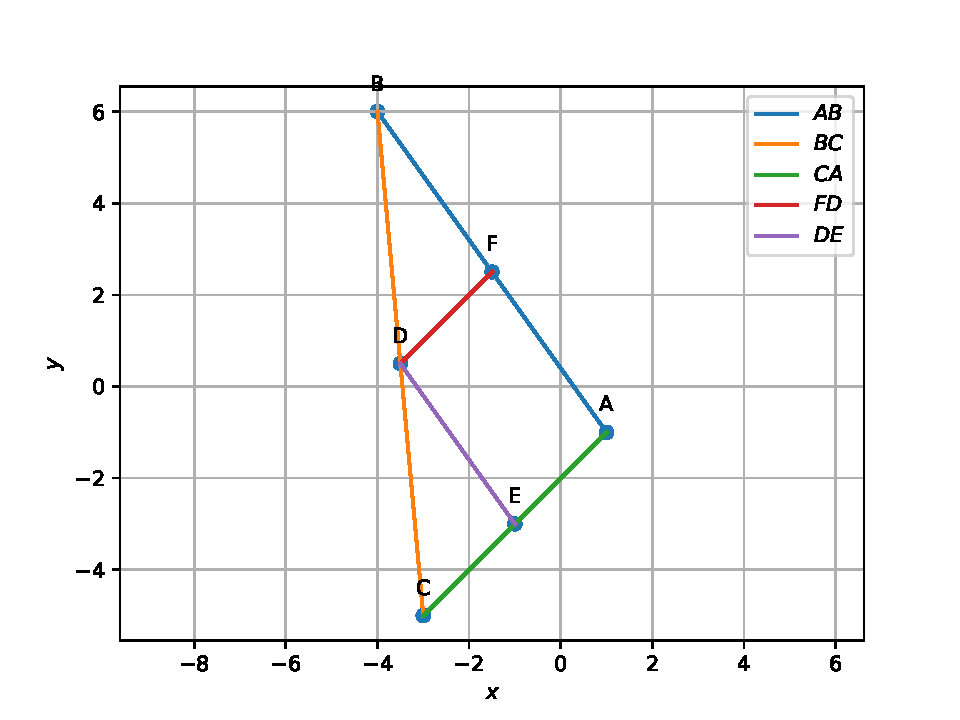
\includegraphics[width=0.75\columnwidth]{figs/triangle/pgm.pdf}
\caption{$AFDE$ forms a parallelogram in triangle ABC}
\label{fig:Triangle-pgm}
\end{figure}






















\item   Points $\vec{A}, \vec{B}, \vec{C}$ are defined to be collinear if 
		\begin{align}
			\label{eq:app-app-line-rank}
			\rank{\myvec{1 & 1 & 1 \\ \vec{A}& \vec{B}&\vec{C}}} = 2
		\end{align}
Are the given points in
			\eqref{eq:app-tri-pts}
collinear?
\\
\solution 
From 
			\eqref{eq:app-tri-pts},
\begin{align}
    \label{eq:app-1.1.3,2}
\myvec{
    1 & 1 & 1\\
    \vec{A} & \vec{B} & \vec{C} \\
    } 
    =
    %\label{eq:app-matthrowoperations}
    \myvec{
    1 & 1 & 1
    \\
    1 & -4 & -3
    \\
    -1 & 6 & -5
    }
     \xleftrightarrow[]{R_3 \leftarrow R_3+R_2}
    \myvec{
    1 & 1 & 1
    \\
    1 & -4 & -3
    \\
    0 & 2 & -8 
    }
    \\
     \xleftrightarrow[]{R_2\leftarrow R_1-R_2}
    \myvec{
    1 & 1 & 1
    \\
    0 & 5 & 4
    \\
    0 & 2 & -8 
    }
     \xleftrightarrow[]{R_3\leftarrow R_3-\frac{2}{5}R_2}
    \myvec{
    1 & 1 & 1
    \\
    0 & 5 & 4
    \\
    0 & 0 & \frac{-48}{5}
    }
\end{align}
There are no zero rows. So,
\begin{align}
    \text{rank}\myvec{
    1 & 1 & 1\\
    \vec{A} & \vec{B} & \vec{C} \\
    } &= 3 
\end{align}  
Hence,  the points $\vec{A},\vec{B},\vec{C}$ are not collinear. 
This is visible in 
\figref{fig1:Triangle}.
\begin{figure}[H]
\centering
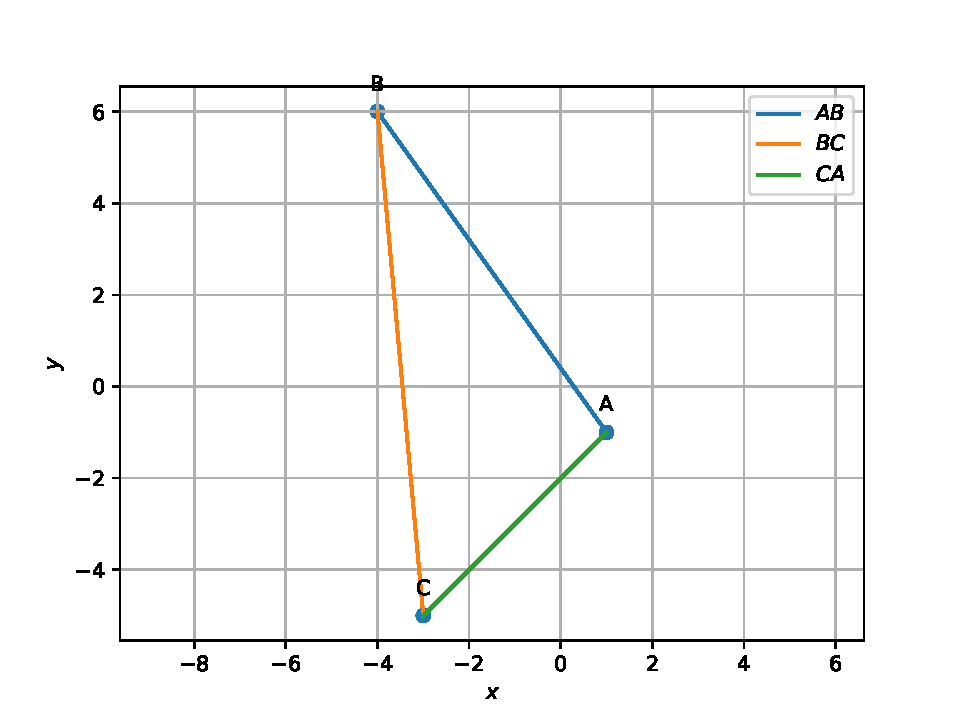
\includegraphics[width=0.75\columnwidth]{figs/triangle/vector.pdf}
\caption{$\triangle ABC$}
\label{fig1:Triangle}
\end{figure}
% \\		\\ \solution 
\begin{align}
    \vec{A}-\vec{F}&=\myvec{1\\-1}-\myvec{\frac{-3}{2}\\\frac{5}{2}}
    =\myvec{\frac{5}{2}\\\frac{-7}{2}}
    \\
    \vec{E}-\vec{D}&=\myvec{-1\\-3}-\myvec{\frac{-7}{2}\\\frac{1}{2}}
    =\myvec{\frac{5}{2}\\\frac{-7}{2}}
    \\
	\implies	\vec{A}-\vec{F} &= \vec{E}-\vec{D}
\end{align}
See \figref{fig:Triangle-pgm}, 
\begin{figure}
\centering
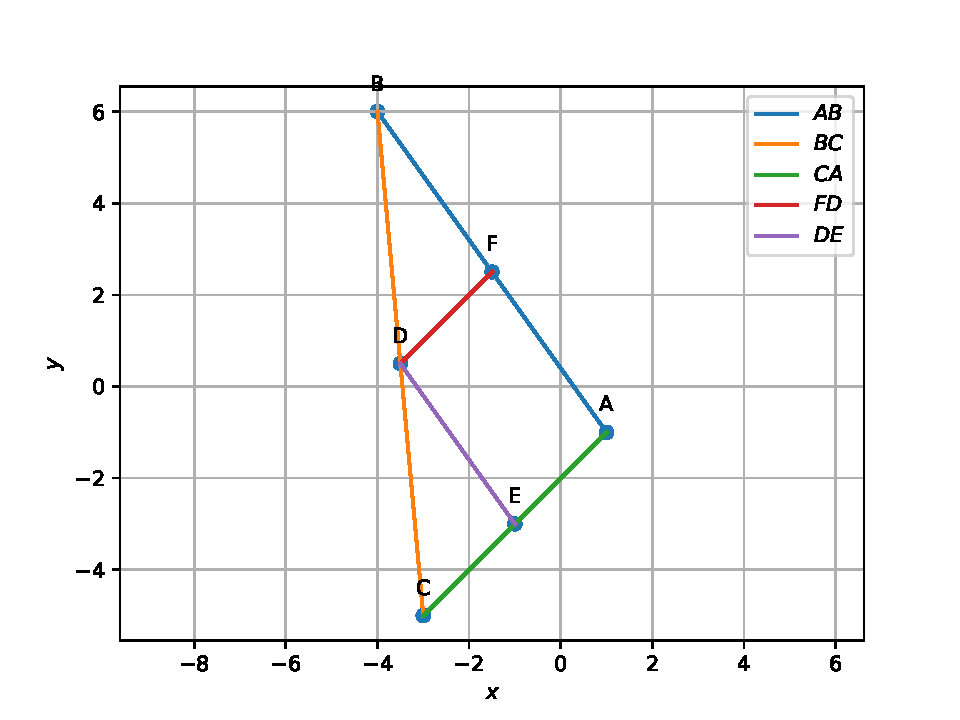
\includegraphics[width=0.75\columnwidth]{figs/triangle/pgm.pdf}
\caption{$AFDE$ forms a parallelogram in triangle ABC}
\label{fig:Triangle-pgm}
\end{figure}






















\item The parameteric form of the equation  of $AB$ is 
		\begin{align}
			\label{eq:app-geo-param}
			\vec{x}=\vec{A}+k\vec{m} \quad k \ne 0,
		\end{align}
		where
		\begin{align}
\vec{m}=\vec{B}-\vec{A}
		\end{align}
is the direction vector of $AB$.
Find the parameteric equations of $AB, BC$ and $CA$.
\\
\solution
From 
			\eqref{eq:app-geo-param} and
		\eqref{eq:app-geo-dir-vec-ab},
the parametric equation for $AB$ is given by
\begin{align}
AB: \vec{x} = &\myvec{1\\-1} + k \myvec{-5\\7}
\end{align}
Similarly, from 
		\eqref{eq:app-geo-dir-vec-bc} and
		\eqref{eq:app-geo-dir-vec-ca},
\begin{align}
BC: \vec{x} = &\myvec{-4\\6} + k \myvec{1\\-11}\\
CA: \vec{x} = &\myvec{-3\\-5} + k \myvec{4\\4}
\end{align}

%		\\ \solution 
\begin{align}
    \vec{A}-\vec{F}&=\myvec{1\\-1}-\myvec{\frac{-3}{2}\\\frac{5}{2}}
    =\myvec{\frac{5}{2}\\\frac{-7}{2}}
    \\
    \vec{E}-\vec{D}&=\myvec{-1\\-3}-\myvec{\frac{-7}{2}\\\frac{1}{2}}
    =\myvec{\frac{5}{2}\\\frac{-7}{2}}
    \\
	\implies	\vec{A}-\vec{F} &= \vec{E}-\vec{D}
\end{align}
See \figref{fig:Triangle-pgm}, 
\begin{figure}
\centering
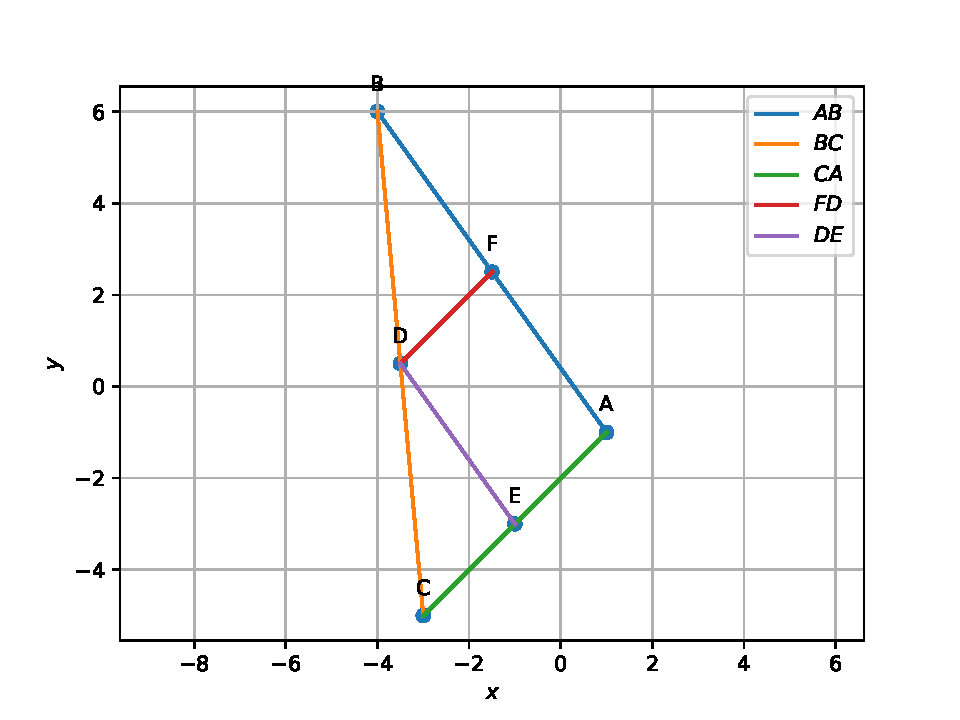
\includegraphics[width=0.75\columnwidth]{figs/triangle/pgm.pdf}
\caption{$AFDE$ forms a parallelogram in triangle ABC}
\label{fig:Triangle-pgm}
\end{figure}






















\item The normal form of the equation of $AB$  is 
		\begin{align}
			\label{eq:app-geo-normal}
			\vec{n}^{\top}\brak{	\vec{x}-\vec{A}} = 0
		\end{align}
		where 
		\begin{align}
			\vec{n}^{\top}\vec{m}&=\vec{n}^{\top}\brak{\vec{B}-\vec{A}} = 0
			\\
			\text{or, } \vec{n}&=\myvec{0 & 1 \\ -1 & 0} \vec{m}
			\label{eq:app-geo-norm-vec}
		\end{align}
Find the normal form of the equations of $AB, BC$ and $CA$.
\\
\solution
\begin{enumerate}
	\item
From
		\eqref{eq:app-geo-dir-vec-bc}, 
the direction vector of side $\vec{BC}$ is
\begin{align}
\vec{m}
	&=\myvec{1\\-11}
	\\
\implies \vec{n} &= \myvec{0 & 1\\
  -1 & 0}\myvec{1\\-11}
 = \myvec{-11\\-1}
		\label{eq:app-geo-norm-vec-bc}
\end{align}
from 
			\eqref{eq:app-geo-norm-vec}.
Hence, from 
			\eqref{eq:app-geo-normal},
the normal equation of side $BC$ is 
\begin{align}
	\vec{n}^{\top}\brak{	\vec{x}-\vec{B}} &= 0
			\\
\implies    \myvec{-11 & -1}\vec{x}&=\myvec{-11 & -1}\myvec{-4\\6}\\
    \implies
BC: \quad    \myvec{11 & 1}\vec{x}&=-38
\end{align}
\item Similarly, for $AB$,
from 
		\eqref{eq:app-geo-dir-vec-ab}, 
\begin{align}
	\vec{m} &= \myvec{-5\\7}
	\\
\implies        \vec{n} 
                &= \myvec{0&1\\-1&0}\myvec{-5\\7}
                = \myvec{7\\5}
		\label{eq:app-geo-norm-vec-ab}
\end{align}
and 
\begin{align}
	\vec{n}^{\top}\brak{	\vec{x}-\vec{A}} &= 0
	\\
	\implies
                AB: \quad  \vec{n}^{\top}\vec{x} &= \myvec{7&5}\myvec{1\\-1}\\    
       \implies\myvec{7&5}\vec{x} &= 2
\end{align}
\item For 
$CA$, 
from 
		\eqref{eq:app-geo-dir-vec-ca}, 
\begin{align}
\vec{m} &= \myvec{1 \\ 1}
\\
		\label{eq:app-geo-norm-vec-ca}
\implies \vec{n} 
&= \myvec{0&1 \\ -1&0}\myvec{1 \\ 1}
= \myvec{1 \\ -1}\\
\\
\implies	\vec{n}^{\top}\brak{	\vec{x}-\vec{C}} &= 0
\\
\implies \myvec{1&-1}{\vec{x}} &= \myvec{1&-1}\myvec{-3 \\ -5} 
= 2 
\end{align}
\end{enumerate}

%\begin{enumerate}
	\item
From
		\eqref{eq:geo-dir-vec-bc}, 
the direction vector of side $\vec{BC}$ is
\begin{align}
\vec{m}
	&=\myvec{1\\-11}
	\\
\implies \vec{n} &= \myvec{0 & 1\\
  -1 & 0}\myvec{1\\-11}
 = \myvec{-11\\-1}
		\label{eq:geo-norm-vec-bc}
\end{align}
from 
			\eqref{eq:geo-norm-vec}.
Hence, from 
			\eqref{eq:geo-normal},
the normal equation of side $BC$ is 
\begin{align}
	\vec{n}^{\top}\brak{	\vec{x}-\vec{B}} &= 0
			\\
\implies    \myvec{-11 & -1}\vec{x}&=\myvec{-11 & -1}\myvec{-4\\6}\\
    \implies
BC: \quad    \myvec{11 & 1}\vec{x}&=-38
\end{align}
\item Similarly, for $AB$,
from 
		\eqref{eq:geo-dir-vec-ab}, 
\begin{align}
	\vec{m} &= \myvec{-5\\7}
	\\
\implies        \vec{n} 
                &= \myvec{0&1\\-1&0}\myvec{-5\\7}
                = \myvec{7\\5}
		\label{eq:geo-norm-vec-ab}
\end{align}
and 
\begin{align}
	\vec{n}^{\top}\brak{	\vec{x}-\vec{A}} &= 0
	\\
	\implies
                AB: \quad  \vec{n}^{\top}\vec{x} &= \myvec{7&5}\myvec{1\\-1}\\    
       \implies\myvec{7&5}\vec{x} &= 2
\end{align}
\item For 
$CA$, 
from 
		\eqref{eq:geo-dir-vec-ca}, 
\begin{align}
\vec{m} &= \myvec{1 \\ 1}
\\
		\label{eq:geo-norm-vec-ca}
\implies \vec{n} 
&= \myvec{0&1 \\ -1&0}\myvec{1 \\ 1}
= \myvec{1 \\ -1}\\
\\
\implies	\vec{n}^{\top}\brak{	\vec{x}-\vec{C}} &= 0
\\
\implies \myvec{1&-1}{\vec{x}} &= \myvec{1&-1}\myvec{-3 \\ -5} 
= 2 
\end{align}
\end{enumerate}


\item The area of $\triangle ABC$ is defined as
		\begin{align}
			\label{eq:app-tri-area-cross}
			\frac{1}{2}\norm{{\brak{\vec{A}-\vec{B}}\times \brak{\vec{A}-\vec{C}}}}
		\end{align}
		where
		\begin{align}
			\vec{A}\times\vec{B} \triangleq \mydet{1 & -4 \\-1 & 6}
		\end{align}
		Find the area of $\triangle ABC$.\\
\solution
From
		\eqref{eq:app-geo-dir-vec-ab}
		and
		\eqref{eq:app-geo-dir-vec-ca},
\begin{align}
	\vec{A}-\vec{B}=\myvec{5\\-7},
	\vec{A}-\vec{C}&=\myvec{4\\4}\\
\implies (\vec{A}-\vec{B})\times(\vec{A}-\vec{C}) &=\mydet{5 & 4\\-7 & 4}\\
&=5\times 4-4\times (-7)\\&=48\\
\implies\frac{1}{2}\norm{(\vec{A}-\vec{B})\times(\vec{A}-\vec{C})}&=\frac{48}{2}=24
\end{align}
which is the desired area.

%  		\\ \solution 
\begin{align}
    \vec{A}-\vec{F}&=\myvec{1\\-1}-\myvec{\frac{-3}{2}\\\frac{5}{2}}
    =\myvec{\frac{5}{2}\\\frac{-7}{2}}
    \\
    \vec{E}-\vec{D}&=\myvec{-1\\-3}-\myvec{\frac{-7}{2}\\\frac{1}{2}}
    =\myvec{\frac{5}{2}\\\frac{-7}{2}}
    \\
	\implies	\vec{A}-\vec{F} &= \vec{E}-\vec{D}
\end{align}
See \figref{fig:Triangle-pgm}, 
\begin{figure}
\centering
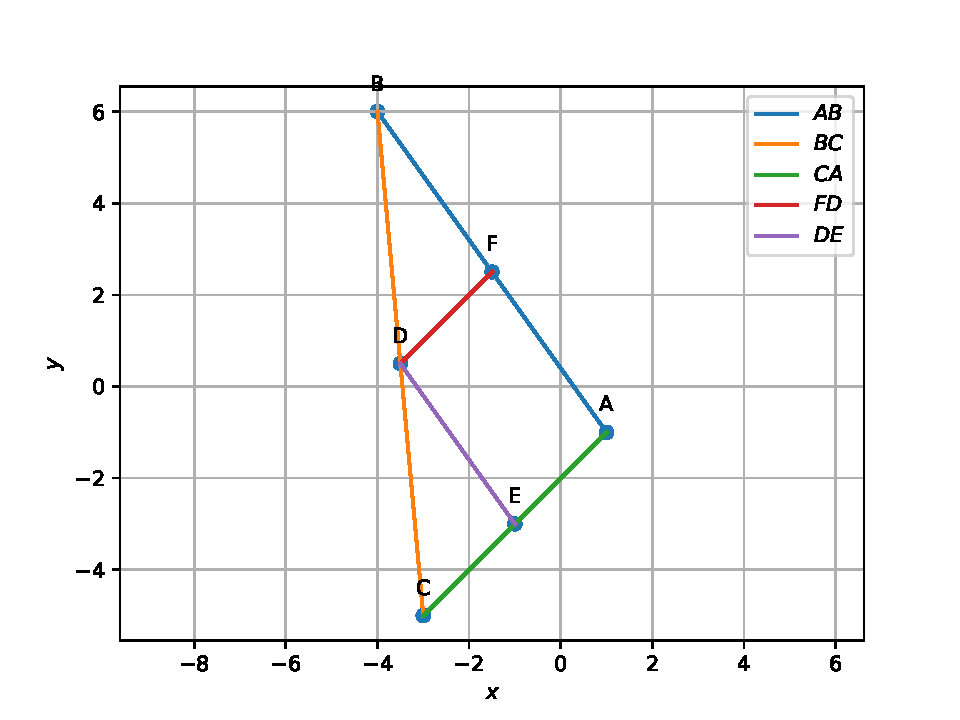
\includegraphics[width=0.75\columnwidth]{figs/triangle/pgm.pdf}
\caption{$AFDE$ forms a parallelogram in triangle ABC}
\label{fig:Triangle-pgm}
\end{figure}






















	\item Find the angles $A, B, C$ if 
%    \label{prop:angle2d}
  \begin{align}
    \label{eq:app-angle2d}
			\cos A \triangleq 
\frac{\brak{\vec{B}-\vec{A}}^{\top}{\vec{C}-\vec{A}}}{\norm{\vec{B}-\vec{A}}\norm{\vec{C}-\vec{A}}}
  \end{align}\\
  \solution
\begin{enumerate}
	\item From 
		\eqref{eq:app-geo-dir-vec-ab},
		\eqref{eq:app-geo-dir-vec-ca},
		\eqref{eq:app-geo-norm-ab}
		and
		\eqref{eq:app-geo-norm-ca}
\begin{align}
	(\vec{B}-\vec{A})^{\top}(\vec{C}-\vec{A})&=\myvec{-5&7}\myvec{-4\\-4}\\
	&=-8
	\\
	\implies
	\cos{A}&= \frac{-8}{\sqrt{74} \sqrt{32}}
	= \frac{-1}{\sqrt{37}}\\
	\implies A&=\cos^{-1}{\frac{-1}{\sqrt{37}}}
\end{align}
	\item From 
		\eqref{eq:app-geo-dir-vec-ab},
		\eqref{eq:app-geo-dir-vec-bc},
		\eqref{eq:app-geo-norm-ab}
		and
		\eqref{eq:app-geo-norm-bc}
\begin{align}
	(\vec{C}-\vec{B})^{\top}(\vec{A}-\vec{B})&=\myvec{1&-11}\myvec{5\\-7}\\
	&= 82
	\\
	\implies
	\cos{B}&= \frac{82}{\sqrt{74} \sqrt{122}}
	= \frac{41}{\sqrt{2257}}\\
	\implies B&=\cos^{-1}{\frac{41}{\sqrt{2257}}}
\end{align}
	\item From 
		\eqref{eq:app-geo-dir-vec-bc},
		\eqref{eq:app-geo-dir-vec-ca},
		\eqref{eq:app-geo-norm-bc}
		and
		\eqref{eq:app-geo-norm-ca}
\begin{align}
	(\vec{A}-\vec{C})^{\top}(\vec{B}-\vec{C})&=\myvec{4&4}\myvec{-1\\11}\\
	&=40
	\\
\implies	\cos{C}&= \frac{40}{\sqrt{32} \sqrt{122}}
	= \frac{5}{\sqrt{61}}\\
	\implies C&=\cos^{-1}{\frac{5}{\sqrt{61}}}
\end{align}

\end{enumerate}
%  	\\ \solution 
\begin{align}
    \vec{A}-\vec{F}&=\myvec{1\\-1}-\myvec{\frac{-3}{2}\\\frac{5}{2}}
    =\myvec{\frac{5}{2}\\\frac{-7}{2}}
    \\
    \vec{E}-\vec{D}&=\myvec{-1\\-3}-\myvec{\frac{-7}{2}\\\frac{1}{2}}
    =\myvec{\frac{5}{2}\\\frac{-7}{2}}
    \\
	\implies	\vec{A}-\vec{F} &= \vec{E}-\vec{D}
\end{align}
See \figref{fig:Triangle-pgm}, 
\begin{figure}
\centering
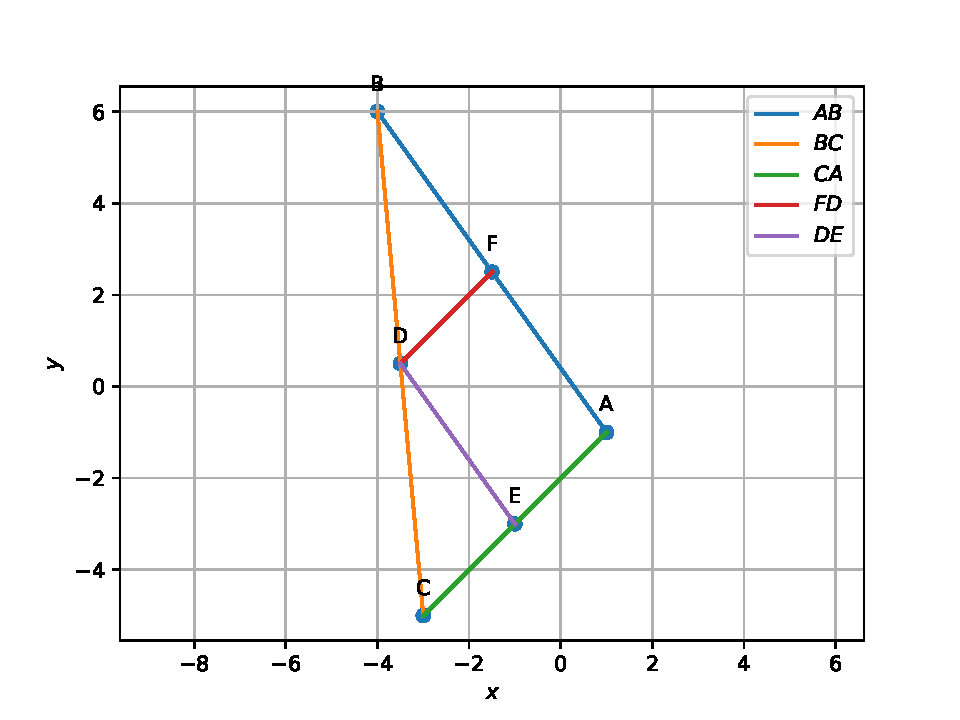
\includegraphics[width=0.75\columnwidth]{figs/triangle/pgm.pdf}
\caption{$AFDE$ forms a parallelogram in triangle ABC}
\label{fig:Triangle-pgm}
\end{figure}






















All codes for this section are available at
\begin{lstlisting}
	codes/triangle/sides.py
\end{lstlisting}
\end{enumerate}

\item If the points $\vec{A}(6,  1),  \vec{B}(8,  2),  \vec{C}(9,  4)$ and $\vec{D}(p,  3)$ are the vertices of a parallelogram,  taken in order,  find the value of $p$.
\label{10/7/0/10}
\item 
If $(1,  2),  (4,  y),  (x,  6)$ and $(3,  5)$ are the vertices of a parallelogram taken in order,  find $x$ and $y$.
\label{10/7/2/6}
\item The fourth vertex $\vec{D}$ of a parallelogram $ABCD$ whose three vertices are
	$\vec{A} (–2,  3),  \vec{B} (6,  7)$ and  $\vec{C} (8,  3)$ is
\item Verify if the points $\vec{A}(4, 3),  \vec{B}(6, 4), \vec{C}(5, -6)$  and  $\vec{D}(-3, 5)$ are the vertices of a parallelogram.
\item A girl walks 4 km towards west,  then she walks 3 km in a direction 30$^{\circ}$ east of north and stops. Determine the girl's displacement from her initial point of departure.\\
	\solution
		\iffalse
\documentclass[10pt]{article}
\usepackage{graphicx}
\def\inputGnumericTable{}
\usepackage[latin1]{inputenc}
\usepackage{fullpage}
\usepackage{color}
\usepackage{array}
\usepackage{longtable}
\usepackage{calc}
\usepackage{multirow}
\usepackage{hhline}
\usepackage{ifthen}
\usepackage{amsmath}
\usepackage[none]{hyphenat}
\usepackage{listings}
\usepackage[english]{babel}
\usepackage{siunitx}
\usepackage{caption}
\usepackage{booktabs}
\usepackage{array}
\usepackage{extarrows}
\usepackage{enumerate}
\usepackage{enumitem}
\usepackage{amsmath}
\usepackage{commath}
\usepackage{gensymb}
\usepackage{amssymb}
\usepackage{multicol}
%\usepackage[utf8]{inputenc}
\lstset{
 frame=single,
 breaklines=true
}
\usepackage{hyperref}
\usepackage[margin=0.65in]{geometry}	 
%\usepackage{exsheets}% also loads the `tasks' package
\usepackage{atbegshi}
\AtBeginDocument{\AtBeginShipoutNext{\AtBeginShipoutDiscard}}

%new macro definitions
\renewcommand{\labelenumi}{(\roman{enumi})}
\newcommand{\mydet}[1]{\ensuremath{\begin{vmatrix}#1\end{vmatrix}}}
\providecommand{\brak}[1]{\ensuremath{\left(#1\right)}}
\newcommand{\solution}{\noindent \textbf{Solution: }}
\newcommand{\myvec}[1]{\ensuremath{\begin{pmatrix}#1\end{pmatrix}}}
\newenvironment{amatrix}[1]{%
	\left(\begin{array}{@{}*{#1}{c}|c@{}}
}{%
	\end{array}\right)
}

\newcommand{\myaugvec}[2]{\ensuremath{\begin{amatrix}{#1}#2\end{amatrix}}}
\providecommand{\norm}[1]{\left\1Vert#1\right\rVert}
\let\vec\mathbf{}


%\SetEnumitemKey{twocol}{
% before=\raggedcolumns\begin{multicols}{2},
% after=\end{multicols}}
%\SetEnumitemKey{fourcol}{
% before=\raggedcolumns\begin{multicols}{4},
% after=\end{multicols}} 


\begin{document}
\begin{center}
\title{\textbf{TRIANGLES}}
\date{\vspace{-5ex}}
\maketitle
\end{center}
\section*{9$^{th}$Math - Chapter 7}
This is Problem-8 from Exercise 7.1\\\\


\section*{\large Construction:}
\fi
The input parameters for construction
	are available in Table \ref{tab:chapters/9/7/1/8/table}.
\begin{table}[H]
	\centering
	%\subimport{../chapters/9/7/1/8/tables/}{table.tex}
     %%%%%%%%%%%%%%%%%%%%%%%%%%%%%%%%%%%%%%%%%%%%%%%%%%%%%%%%%%%%%%%%%%%%%%
%%                                                                  %%
%%  This is the header of a LaTeX2e file exported from Gnumeric.    %%
%%                                                                  %%
%%  This file can be compiled as it stands or included in another   %%
%%  LaTeX document. The table is based on the longtable package so  %%
%%  the longtable options (headers, footers...) can be set in the   %%
%%  preamble section below (see PRAMBLE).                           %%
%%                                                                  %%
%%  To include the file in another, the following two lines must be %%
%%  in the including file:                                          %%
%%        \def\inputGnumericTable{}                                 %%
%%  at the beginning of the file and:                               %%
%%        \input{name-of-this-file.tex}                             %%
%%  where the table is to be placed. Note also that the including   %%
%%  file must use the following packages for the table to be        %%
%%  rendered correctly:                                             %%
%%    \usepackage[latin1]{inputenc}                                 %%
%%    \usepackage{color}                                            %%
%%    \usepackage{array}                                            %%
%%    \usepackage{longtable}                                        %%
%%    \usepackage{calc}                                             %%
%%    \usepackage{multirow}                                         %%
%%    \usepackage{hhline}                                           %%
%%    \usepackage{ifthen}                                           %%
%%  optionally (for landscape tables embedded in another document): %%
%%    \usepackage{lscape}                                           %%
%%                                                                  %%
%%%%%%%%%%%%%%%%%%%%%%%%%%%%%%%%%%%%%%%%%%%%%%%%%%%%%%%%%%%%%%%%%%%%%



%%  This section checks if we are begin input into another file or  %%
%%  the file will be compiled alone. First use a macro taken from   %%
%%  the TeXbook ex 7.7 (suggestion of Han-Wen Nienhuys).            %%
\def\ifundefined#1{\expandafter\ifx\csname#1\endcsname\relax}


%%  Check for the \def token for inputed files. If it is not        %%
%%  defined, the file will be processed as a standalone and the     %%
%%  preamble will be used.                                          %%
\ifundefined{inputGnumericTable}

%%  We must be able to close or not the document at the end.        %%
	\def\gnumericTableEnd{\end{document}}


%%%%%%%%%%%%%%%%%%%%%%%%%%%%%%%%%%%%%%%%%%%%%%%%%%%%%%%%%%%%%%%%%%%%%%
%%                                                                  %%
%%  This is the PREAMBLE. Change these values to get the right      %%
%%  paper size and other niceties.                                  %%
%%                                                                  %%
%%%%%%%%%%%%%%%%%%%%%%%%%%%%%%%%%%%%%%%%%%%%%%%%%%%%%%%%%%%%%%%%%%%%%%

	\documentclass[12pt%
			  %,landscape%
                    ]{report}
       \usepackage[latin1]{inputenc}
       \usepackage{fullpage}
       \usepackage{color}
       \usepackage{array}
       \usepackage{longtable}
       \usepackage{calc}
       \usepackage{multirow}
       \usepackage{hhline}
       \usepackage{ifthen}
       \usepackage{gensymb}
       \usepackage{graphicx}
\usepackage{amsmath}
\usepackage{mathtools}
\newcommand{\mydet}[1]{\ensuremath{\begin{vmatrix}#1\end{vmatrix}}}
\providecommand{\brak}[1]{\ensuremath{\left(#1\right)}}
\providecommand{\norm}[1]{\left\lVert#1\right\rVert}
\newcommand{\solution}{\noindent \textbf{Solution: }}
\newcommand{\myvec}[1]{\ensuremath{\begin{pmatrix}#1\end{pmatrix}}}
\let\vec\mathbf
	\begin{document}


%%  End of the preamble for the standalone. The next section is for %%
%%  documents which are included into other LaTeX2e files.          %%
\else

%%  We are not a stand alone document. For a regular able, we will %%
%%  have no preamble and only define the closing to mean nothing.   %%
    \def\gnumericTableEnd{}

%%  If we want landscape mode in an embedded document, comment out  %%
%%  the line above and uncomment the two below. The table will      %%
%%  begin on a new page and run in landscape mode.                  %%
%       \def\gnumericTableEnd{\end{landscape}}
%       \begin{landscape}


%%  End of the else clause for this file being \input.              %%
\fi

%%%%%%%%%%%%%%%%%%%%%%%%%%%%%%%%%%%%%%%%%%%%%%%%%%%%%%%%%%%%%%%%%%%%%%
%%                                                                  %%
%%  The rest is the gnumeric table, except for the closing          %%
%%  statement. Changes below will alter the table's appearance.     %%
%%                                                                  %%
%%%%%%%%%%%%%%%%%%%%%%%%%%%%%%%%%%%%%%%%%%%%%%%%%%%%%%%%%%%%%%%%%%%%%%
\providecommand{\gnumericmathit}[1]{#1} 
%%  Uncomment the next line if you would like your numbers to be in %%
%%  italics if they are italizised in the gnumeric table.           %%
%\renewcommand{\gnumericmathit}[1]{\mathit{#1}}
\providecommand{\gnumericPB}[1]%
{\let\gnumericTemp=\\#1\let\\=\gnumericTemp\hspace{0pt}}
 \ifundefined{gnumericTableWidthDefined}
        \newlength{\gnumericTableWidth}
        \newlength{\gnumericTableWidthComplete}
        \newlength{\gnumericMultiRowLength}
        \global\def\gnumericTableWidthDefined{}
 \fi
%% The following setting protects this code from babel shorthands.  %%
 \ifthenelse{\isundefined{\languageshorthands}}{}{\languageshorthands{english}}
%%  The default table format retains the relative column widths of  %%
%%  gnumeric. They can easily be changed to c, r or l. In that case %%
%%  you may want to comment out the next line and uncomment the one %%
%%  thereafter                                                      %%
\providecommand\gnumbox{\makebox[0pt]}
%%\providecommand\gnumbox[1][]{\makebox}

%% to adjust positions in multirow situations                       %%
\setlength{\bigstrutjot}{\jot}
\setlength{\extrarowheight}{\doublerulesep}

%%  The \setlongtables command keeps column widths the same across  %%
%%  pages. Simply comment out next line for varying column widths.  %%
\setlongtables

\setlength\gnumericTableWidth{%
	40pt+%
	35pt+%
	210pt+%
0pt}
\def\gumericNumCols{3}
\setlength\gnumericTableWidthComplete{\gnumericTableWidth+%
         \tabcolsep*\gumericNumCols*2+\arrayrulewidth*\gumericNumCols}
\ifthenelse{\lengthtest{\gnumericTableWidthComplete > \linewidth}}%
         {\def\gnumericScale{\ratio{\linewidth-%
                        \tabcolsep*\gumericNumCols*2-%
                        \arrayrulewidth*\gumericNumCols}%
{\gnumericTableWidth}}}%
{\def\gnumericScale{1}}

%%%%%%%%%%%%%%%%%%%%%%%%%%%%%%%%%%%%%%%%%%%%%%%%%%%%%%%%%%%%%%%%%%%%%%
%%                                                                  %%
%% The following are the widths of the various columns. We are      %%
%% defining them here because then they are easier to change.       %%
%% Depending on the cell formats we may use them more than once.    %%
%%                                                                  %%
%%%%%%%%%%%%%%%%%%%%%%%%%%%%%%%%%%%%%%%%%%%%%%%%%%%%%%%%%%%%%%%%%%%%%%

\ifthenelse{\isundefined{\gnumericColA}}{\newlength{\gnumericColA}}{}\settowidth{\gnumericColA}{\begin{tabular}{@{}p{40pt*\gnumericScale}@{}}x\end{tabular}}
\ifthenelse{\isundefined{\gnumericColB}}{\newlength{\gnumericColB}}{}\settowidth{\gnumericColB}{\begin{tabular}{@{}p{35pt*\gnumericScale}@{}}x\end{tabular}}
\ifthenelse{\isundefined{\gnumericColC}}{\newlength{\gnumericColC}}{}\settowidth{\gnumericColC}{\begin{tabular}{@{}p{65pt*\gnumericScale}@{}}x\end{tabular}}

\begin{longtable}[c]{%
	b{\gnumericColA}%
	b{\gnumericColB}%
	b{\gnumericColC}%
	}

%%%%%%%%%%%%%%%%%%%%%%%%%%%%%%%%%%%%%%%%%%%%%%%%%%%%%%%%%%%%%%%%%%%%%%
%%  The longtable options. (Caption, headers... see Goosens, p.124) %%
%	\caption{The Table Caption.}             \\	%
% \hline	% Across the top of the table.
%%  The rest of these options are table rows which are placed on    %%
%%  the first, last or every page. Use \multicolumn if you want.    %%

%%  Header for the first page.                                      %%
%	\multicolumn{3}{c}{The First Header} \\ \hline 
%	\multicolumn{1}{c}{colTag}	%Column 1
%	&\multicolumn{1}{c}{colTag}	%Column 2
%	&\multicolumn{1}{c}{colTag}	\\ \hline %Last column
%	\endfirsthead

%%  The running header definition.                                  %%
%	\hline
%	\multicolumn{3}{l}{\ldots\small\slshape continued} \\ \hline
%	\multicolumn{1}{c}{colTag}	%Column 1
%	&\multicolumn{1}{c}{colTag}	%Column 2
%	&\multicolumn{1}{c}{colTag}	\\ \hline %Last column
%	\endhead

%%  The running footer definition.                                  %%
%	\hline
%	\multicolumn{3}{r}{\small\slshape continued\ldots} \\
%	\endfoot

%%  The ending footer definition.                                   %%
%	\multicolumn{3}{c}{That's all folks} \\ \hline 
%	\endlastfoot
%%%%%%%%%%%%%%%%%%%%%%%%%%%%%%%%%%%%%%%%%%%%%%%%%%%%%%%%%%%%%%%%%%%%%%

\hhline{|-|-|-}
	 \multicolumn{1}{|p{\gnumericColA}|}%
	{\gnumericPB{\raggedright}\gnumbox[l]{\textbf{Symbol}}}
	&\multicolumn{1}{p{\gnumericColB}|}%
	{\gnumericPB{\raggedright}\gnumbox[l]{\textbf{Values}}}
	&\multicolumn{1}{p{\gnumericColC}|}%
	{\gnumericPB{\raggedright}\gnumbox[l]{\textbf{Description}}}
\\
\hhline{|---|}
	 \multicolumn{1}{|p{\gnumericColA}|}%
	{\gnumericPB{\raggedright}\gnumbox[l]{$r$}}
	&\multicolumn{1}{p{\gnumericColB}|}%
	{\gnumericPB{\raggedright}\gnumbox[l]{2}}
	&\multicolumn{1}{p{\gnumericColC}|}%
	{\gnumericPB{\raggedright}\gnumbox[l]{radius}}
\\
\hhline{|---|}
	 \multicolumn{1}{|p{\gnumericColA}|}%
	{\gnumericPB{\raggedright}\gnumbox[l]{$\vec{O}$}}
	&\multicolumn{1}{p{\gnumericColB}|}%
	{\gnumericPB{\raggedright}\gnumbox[l]{$\myvec{0\\0}$}}
	&\multicolumn{1}{p{\gnumericColC}|}%
	{\gnumericPB{\raggedright}\gnumbox[l]{center}}
\\
\hhline{|---|}
\end{longtable}

\ifthenelse{\isundefined{\languageshorthands}}{}{\languageshorthands{\languagename}}
\gnumericTableEnd%t

	\caption{}
	\label{tab:chapters/9/7/1/8/table}
\end{table}
Thus, 
\begin{align}
	\vec{A}=\myvec{0\\b},\,
	\vec{B}=\myvec{a\\0},\,
	\vec{C}=\myvec{0\\0}
\end{align}
yielding
\begin{align}
	\vec{M}&=\frac{\vec{A}+\vec{B}}{2}=\frac{1}{2}\myvec{a\\b}
\end{align}
Also, 
\begin{align}
	\vec{M}&=\frac{\vec{C}+\vec{D}}{2}\\
	\implies \vec{D}&=2\vec{M}-\vec{C}=\myvec{a\\b}
\end{align}
\iffalse
\solution
Given
\begin{align}
	\vec{M}&=\frac{\vec{A}+\vec{B}}{2}
	\label{eq:chapters/9/7/1/8/1}\\
	\vec{D}-\vec{M}&=\vec{C}-\vec{M}
	\label{eq:chapters/9/7/1/8/2}\\
	\angle ACB&=90\degree
\end{align}
\textbf{Proof:} From Figure \ref{fig:chapters/9/7/1/8/1}
\fi
Thus,
\begin{align}
	\brak{\vec{D}-\vec{B}}^{\top}\brak{\vec{B}-\vec{C}} &= \myvec{0 & b}\myvec{a\\0}=0\\
	\implies BD & \perp BC\\
\end{align}
Also, 
\begin{align}
	\norm{\vec{A}-\vec{B}}&=\norm{\myvec{-a\\b}}\\
	\norm{\vec{C}-\vec{D}}&=\norm{\myvec{-a\\-b}}\\
	\implies \norm{\vec{A}-\vec{B}} &= \norm{\vec{C}-\vec{D}}\\
	\text{ or, } AB &= CD
	\label{eq:chapters/9/7/1/8/3}	
\end{align}
From \eqref{eq:chapters/9/7/1/8/3}
\begin{align}
	\implies CM = \frac{1}{2}CD = \frac{1}{2}AB 
\end{align}
See Fig. 
\ref{fig:chapters/9/7/1/8/1}.
\begin{figure}[H]
	\begin{center}
		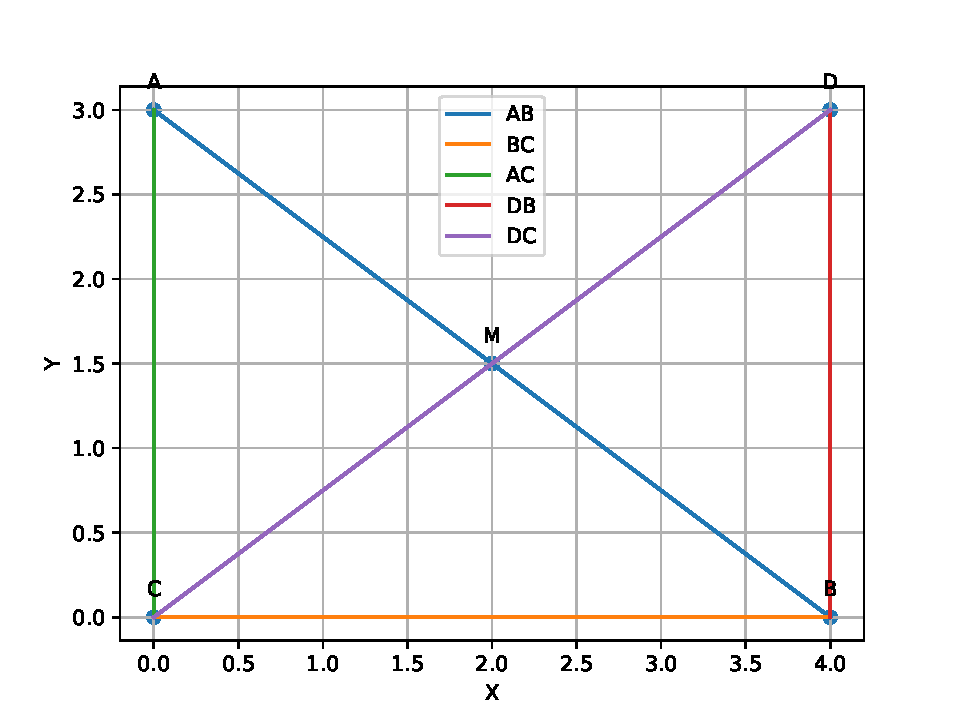
\includegraphics[width=0.75\columnwidth]{./chapters/9/7/1/8/figs/fig.pdf}
	\end{center}
\caption{}
\label{fig:chapters/9/7/1/8/1}
\end{figure}


\item $(-1, 2, 1),  (1, -2, 5),  (4, -7, 8)$ and $(2, -3, 4)$ are the vertices of a parallelogram.
\item Three vertices of a parallelogram $ABCD$ are $\vec{A}(3, -1, 2),  \vec{B}(1, -2, 4)$ and $\vec{C}(-1, 1, 2)$. Find the coordinates of the fourth vertex.
\item If the origin is the centroid of the triangle $PQR$ with vertices $\vec{P}(2a, 2, 6),  \vec{Q}(-4, 3b, -10)$ and $R(8, 14, 2c)$,  then find the values of $a,  b$ and $c$.
\item Find the slope of lines
\begin{enumerate}
\item  Passing through the points $(3, -2)$ and $(-1, 4)$
\item  Passing through the points $(3, -2)$ and $(7, -2)$
\item  passing through the points $(3, -2)$ and $(3, 4)$	
\item  Making inclination of $60\degree$ with the positive direction of x-axis.
\end{enumerate}
\item The centroid of a triangle $ABC$ is at the point $(1, 1, 1)$. If the coordinates of $\vec{A}$ and $\vec{B}$ are $(3, -5, 7)$ and $(-1, 7, -6)$,  respectively find the coordinates of the point $\vec{C}$.
\item Represent graphically a displacement of $40$ km,  $30\degree$ west of south.
	\item Rain is falling vertically with a speed of 35 $m s^{-1}$
. Winds starts blowing after sometime with a speed of 12 $m s^{-1}$ in
east to west direction. In which direction should a boy waiting at a bus stop hold his umbrella ?
%
\item A motorboat is racing towards north at 25 km/h and the water current in that region is 10 km/h in the direction of 60$\degree$ east of south. Find the resultant velocity of the boat.
\item Rain is falling vertically with a speed of 35 $m s^{-1}$
. A woman rides a bicycle with a speed of 12 $ms^{-1}$ in east to west
direction. What is the direction in which she should hold her umbrella ?
\item Rain is falling vertically with a speed of 30 $m s^{-1}$. A woman rides a bicycle with a speed  of 10 $m s^{-1}$ in the north to south direction. What is the direction in which she should
hold her umbrella?
\item A man can swim with a speed of 4.0 km/h in still water. How long does he take to cross a river 1.0 km wide if the river flows steadily at 3.0 km/h and he makes his strokes normal to the river current? How far down the river does he go when he reaches the other bank ?
\item In a harbour,  wind is blowing at the speed of 72 km/h and the flag on the mast of a boat anchored in the harbour flutters along the N-E direction. If the boat starts moving at a speed of 51 km/h to the north,  what is the direction of the flag on the mast of the boat ?
\item In which quadrant or on which axis do each of the points (-2, 4), (3, -1), (-1, 0), (1, 2) and (-3, -5) lie? Verify your answer by locating them on the Cartesian plane.
\item Plot the points $(x, y)$ given in 
\tabref{table:Table of values}.
\begin{table}[H]
	\centering
\begin{tabular}{|c|c|c|c|c|c|}
\hline	
x & -2 & -1 & 0 & 1 & 3\\
\hline
y & 8 & 7 & -1.25 & 3 & -1\\
\hline
\end{tabular}
\caption{}
\label{table:Table of values}
\end{table}
\end{enumerate}
